\documentclass[a4paper]{report}

\usepackage{alltt}
\usepackage{graphicx}
\usepackage{url}
\usepackage[utf8]{inputenc}
\usepackage[magyar]{babel}

\title{RTF támogatás a LibreOffice Writer programban}
\author{Vajna Miklós <vmiklos@frugalware.org>}

\begin{document}

\tableofcontents

\chapter{Vajna Miklós: RTF támogatás a LibreOffice Writer programban}

\section{A Google Summer of Code-ról}

A GSoC egy pályázati lehetőség szervezetek és tanulók számára.  Először
szervezetek pályázhatnak ötletekkel, majd mikor az elfogadott szervezetek
listája publikussá válik, tanulók jelentkezhetnek a szervezeteknél.
Jelentkezéskor általában egy -- a szervezet által kiírt -- ötlet alapján
kidolgozott pályázattal kopognak be a tanulók, de a kreatívabbak teljesen saját
ötlettel is előállhatnak. Mikor lezárult a jelentkezési határidő, a pályázatok
elbírálásra kerülnek, végül publikussá válik a sikeresen beválasztott tanulók
listája.

A program móttója -- \emph{Flip Bits not Burgers} -- arra utal, hogy eredetileg
a cég ezzel azokat a tehetséges fiatalokat kívánta megcélozni, akik egyébként
gyorséttermekben töltötték volna a nyarat, hogy pénzhez jussanak. A
kezdeményezés lehetőséget biztosít arra, hogy szabad szoftver fejlesztéssel
jussanak pénzhez.

A GSoC két ok miatt kerül említésre az előadáson:

\begin{itemize}
\item a bemutatott RTF filterek is hasonló finanszírozásban készültek el,
valamint
\item reklámként is szolgál, hogy jövőre is legyenek olyan tanulók akik a
LibreOffice fejlesztésével szeretnék tölteni nyarukat.
\end{itemize}

\section{A LibreOffice fejlesztésről}

A LibreOffice projekt 2010. szeptember 28-án indult, alapítványi hátterét a The
Document Foundation (röviden TDF) biztosítja. A szabad szoftveres projekt az
OpenOffice.org forkjaként látta meg a napvilágot, a korábban patchset
formájában létező Go-OO folytatásaként.

Fontos különbség, hogy míg a Go-OO a funkciók nagy részét hosszútávon vissza
akarta juttatni az OpenOffice.org-ba, addig a LibreOffice esetén ezt feladták,
így a projekt már a saját útján jár.

Ettől eltekintve persze a nagy kódbázis jelentős része megegyezik, így az
OpenOffice.org projektben szerzett tapasztalatok itt is könnyen
kamatoztathatóak.

Gyakori félreértés, hogy az emberek úgy gondolják: a LibreOffice Java nyelven
íródott, holott ez nincs így. A kód nagy része C++, a maradék többségét valóban
a Java teszi ki, de emellett még számos egyéb nyelven írt kisebb kódokat is
tartalmaz a projekt. (XML, Make, ASM, Yacc, Perl, Python, stb.)

Kedvcsinálóként az előadáson ismertetésre kerülnek azok az első lépések,
melyeket meg kell tennie azon önkénteseknek, akik szeretnének a projekthez
programkóddal hozzájárulni.

\subsection*{Első build}

Az első fordítás három lépésből áll:

\begin{enumerate}
\item forrás letöltése:

\begin{verbatim}
git clone git://anongit.freedesktop.org/libreoffice/core
\end{verbatim}

\item fordítás

\begin{verbatim}
./autogen.sh
make
make dev-install
\end{verbatim}

\item futtatás

\begin{verbatim}
cd install/program
source ./ooenv
./soffice.bin
\end{verbatim}

\end{enumerate}

\subsection*{Inkrementális build}

Mivel egy teljes fordítás sok időt vesz igénybe, a következő kérdés, hogy a
forráskódbeli módosítástól az új futtatható programig hogyan juthatunk el.
Ennek módja, hogy a forráskód számos (jelenleg 226) modulra van osztva, melyek
külön-külön is fordíthatóak.

Például ha a \texttt{writerfilter} modult módosítottuk, akkor lépjünk annak
könyvtárába és futtassuk ott a \texttt{make} programot, aminek határására
futtatáskor már életbe lépnek a változtatásaink.

A gyakorlatban néhány paramétert praktikus alkalmazni:

\begin{itemize}
\item \texttt{-s}: kevesebb kimenet kérése, hogy a hibákat/figyelmeztetéseket könnyebben észrevegyük

\item \texttt{-r}: a beépített implicit szabályok elhagyása, mely gyorsabb működést eredményez

\item \texttt{-j4}: többszálú fordítás (a 4 az aktuális gépen elérhető CPU-k vagy magok számával helyettesítendő)

\item \texttt{dbglevel=2}: a fejlesztést segítő, \texttt{OSL\_TRACE()} kimenetek bekapcsolása

\item \texttt{build}: csak fordítás, unit tesztek futtatásának elhagyása
\end{itemize}

A teljes parancs tehát:

\begin{verbatim}
make -sr -j4 dbglevel=2 build
\end{verbatim}

Aminek segítségével tipikusan 10 másodperc alá szorítható a fordítási idő.
Természetesen az egyes paramétereket mindenki ízlése szerint megválaszthatja.

\subsection*{A projekt mérete}

A LibreOffice az egyik legnagyobb méretű szabad szoftveres projekt. Voltak arra
törekvések, hogy a forráskódot 20-nál is több külön álló tárolóba szétválasszák, de
jelenleg olyan szoros az ezek közötti függés, hogy ez kudarcot vallott: a
fejlesztés során nem vált lehetségessé ténylegesen csak egy-egy alrendszer
módosítása. Ennek következtében jelenleg a módosítások nagy része egyetlen (a \texttt{core})
tárolóban történik.

A \texttt{git clone} végeztével kb. 8 millió kódsorhoz jutunk, a
merevlemezünkön pedig kb. 4 GB helyet veszítünk. A teljes fordítás ideje eltérő
lehet: Linuxon szélső értékként egyrészt a gyakori fordítás (pl. tinderbox) és
\texttt{ccache} használat mellett elérhető kb. 15 perces időigényt lehet
említeni, a másik véglet ha minden nyelv támogatását bekapcsoljuk, akkor még
egy 4 magos gépen is 3-4 óra fordítási idővel kell számoljunk.\footnote{Ha
lassúsági rekordot szeretnénk elérni, próbálkozzunk a fordítással egy manapság
oly divatos netbookon.}

\subsection*{Kollaboráció}

A LibreOffice fejlesztése főként a következő kommunikációs csatornákon keresztül folyik:

\begin{itemize}
\item forráskód kezelés: git
\item napi kommunikáció: IRC, e-mail
\item stratégiai döntések: Technical Steering Call (TSC)
\end{itemize}

\subsection*{RTF filterek}

Filtereknek nevezzük azokat a programmodulokat, melyek a dokumentummodell
betöltését vagy elmentését végzik valamilyen -- lehetőleg szabványosított --
formába. Az cikk szerzője a továbbiakban a Writer alkalmazás RTF import/export
filtereinek elkészítése során szerzett tapasztalatait ill. élményeit ismerteti.

Az RTF formátumot sokan jelentéktelen szabványnak tartják, pedig a maga nemében egyedülálló:

\begin{itemize}
\item Az első verzióját 1987-ben fogadták el, megelőzve az XML-t vagy az ODF-et.
\item Az újabb verziói visszafele kompatibilisak.
\item Időről időre frissül, a jelenlegi (1.9.1-es) szabvány támogatja a beágyazott táblázatokat, OLE objektumokat, stb.
\item Előszeretettel használják sok helyen -- pl. kormányzati űrlapok --, ahol az ODF
még túlságosan újdonságnak számít.
\end{itemize}

Természetesen megvan az a hátránya, hogy az RTF nem egy nyílt szabvány, hanem a
Microsoft adja ki az újabb verziókat.

\section{RTF export fejlesztés}

2010 nyarán egy teljesen új RTF exporter készült el. Az ötlet az volt, hogy az
RTF sok aspektusban hasonlít a doc, ill. docx formátumokra (Microsoft találmány mindhárom), és
a doc/docx exportereknek már van egy közös alapja. A korábban különálló RTF
exporter helyett tehát egy -- erre a közös alapra építkező -- új RTF exporter
készült el.

A szokásos célok (ne okozzon regressziót a régi filterhez képest, legyen
kisebb, nyújtson több funkcionalitást) közül csak a méret csökkentése nem
sikerült, az új funkciók hely-igénye miatt.

Ez az exporter először a Go-OO 3.3 első teszt-kiadásában volt elérhető, azóta
része a LibreOffice-nak. A LibreOffice megszületése előtt része lett az
OpenOffice.org 3.4 bétának is, amiből sajnos azóta se látott a világ stabil
kiadást.\footnote{Aki kíváncsi a fejleményekre, látogasson el az \emph{Apache
OpenOffice.org (incubating)} projekt fejlesztői listájára és kövesse az
eseményeket.} Ettől függetlenül az Oracle híresen szőrszálhasogató QA-én
átjutott az exporter, és ennek során számos hasznos visszajelzést kaptam a cég
mérnökeitől.

Az exportert leginkább azoknak érdemes kipróbálniuk akiknek problémájuk akadt a
régi változattal, de az érdeklődők számára az előadáson példákat mutattam a
következő új funkciókra:

\begin{itemize}
\item könyvjelzőkre mutató oldalszám-hivatkozások
\item karakter tulajdonságok (kiterjesztett térköz, alávágás)
\item OLE objektumok, pl. diagram
\item rajzok
\item űrlapok
\item sorszámozás
\item matematikai kifejezések, szerkesztést lehetővé tevő natív adattal
\item oldaltörések
\item oldalszámozási stílusok, oldalszámozás újraindítása
\item képek Wordpadben
\item post-it mező
\item hasábtörés
\item védett szakaszok
\item beágyazott táblázatok
\item javított tartalomjegyzék
\end{itemize}

Az új funkciók hosszú listája ellenére az új filter se hibamentes,
visszajelzéseket a Freedesktop
Bugzillájába\footnote{\url{http://bugs.freedesktop.org}} kéretik eljuttatni.

\section{RTF import fejlesztés}

Idén nyáron került sor az új RTF importer elkészítésére, mely az exporterhez
hasonló ötleten alapszik: a docx importerhez készült framework
újrahasznosítható lenne több tokenizáló elkészítéséhez \aref{fig:rtf-arch}.
ábrán látható módon.

\vspace{10mm}

\begin{figure}[h!]
\centering
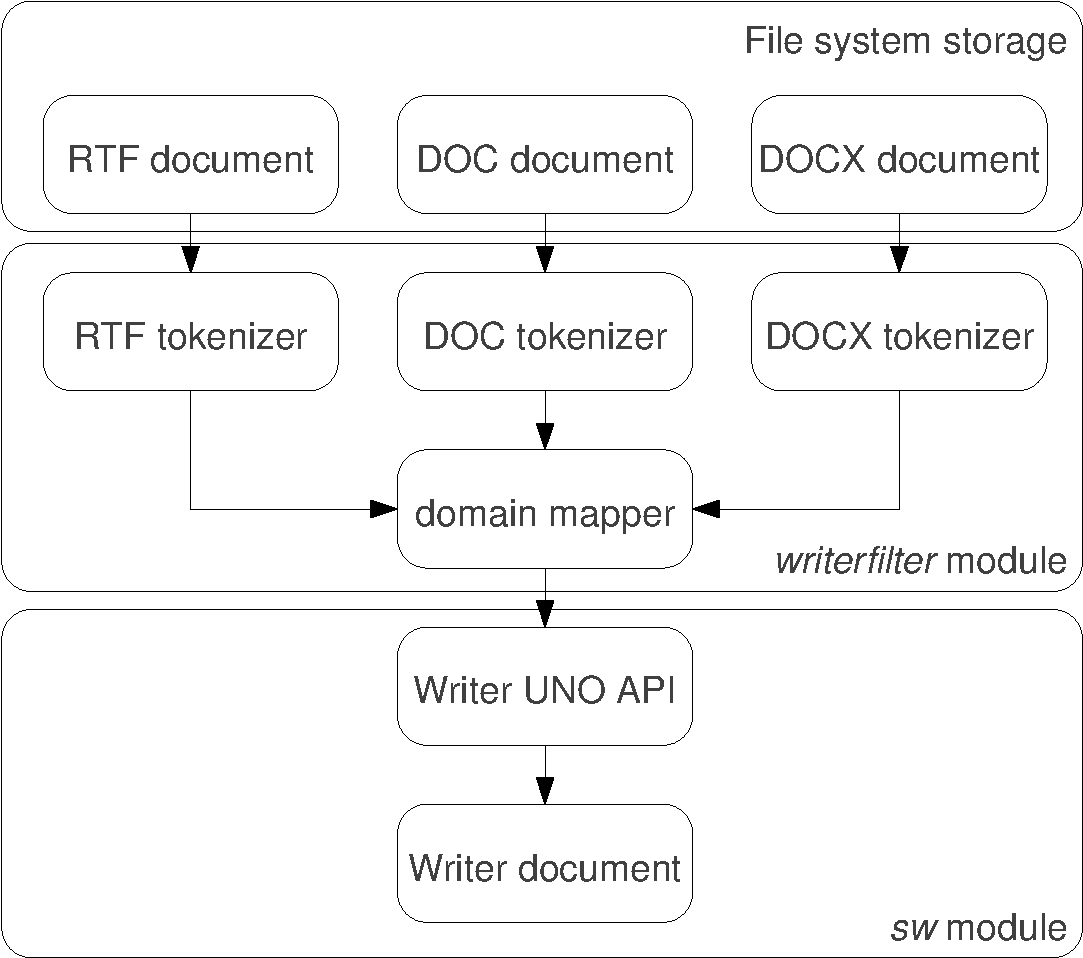
\includegraphics[width=100mm,keepaspectratio]{overview-architecture.pdf}
\caption{Az RTF import filter architektúrája}
\label{fig:rtf-arch}
\end{figure}

Jó példa az így egy helyen megvalósított funkciókra a mezők értelmezése (pl.
oldalszám, annotációk) vagy a Writer oldalstílusai és a Word speciális fejlécei
között.

\subsection*{Tesztelés}

A tesztelés első lépése a csak a tokenizert tesztelő unit teszt elkészítése
volt. A minden fordítás során automatikusan lefutó ellenőrzés a korábbi RTF
importer CVE hibáihoz tartozó teszt dokumentumokat értelmezi. Mivel csak a
tokenizer kerül tesztelésre, a teljes futás kb. 200 ms.

A megoldás szépsége, hogy így már akkor lehetséges a teszteket végrehajtani,
mikor a Writer alkalmazást megvalósító \texttt{sw} modul még nem került
lefordításra.

Természetesen ez a teszt a kézi ellenőrzést nem helyettesíti, hiszen a vizuális
megjelenést nem vizsgálja -- csak azt, hogy a tokenizer elfogadja, vagy
elutasítja az adott dokumentumot.

\subsection*{Új funkciók}

Az export filterhez hasonlóan az importer új funkcióiból is ízelítőt kapnak az
előadás hallgatói. Bemutatásra kerülnek a korábban nem, vagy hiányosan ill. rosszul támogatott
következő elemek importálása:

\begin{itemize}
\item beágyazott táblázatok
\item lábjegyzetek
\item post-it mezők
\item űrlapok
\item rajzok
\item szövegdobozok
\end{itemize}

\subsection*{Hatás a DOCX importra}

A régi RTF importernek néhány funkcióját először azért nem lehetett megvalósítani az új filterben, mert a keretrendszer nem támogatta az adott funkciót. Ezek a módosítások a bekerülésük után a DOCX importert is javították, melyből néhány szintén demonstrálásra került az előadáson:

\begin{itemize}
\item dupla-áthúzás
\item lábjegyzetek újraszámozása
\end{itemize}

\section{Elérhetőségek}

A szerző ezúton is elnézést kér, hogy sok -- a cikkben szereplő -- témát
csak érintőlegesen említett, csak az import és export filterek témáról
vastag könyvet lehetne írni, a cél leginkább a figyelemfelkeltés volt.
Az alábbi linkek további kérdések esetén remélhetőleg segítséget
nyújtanak.

\begin{itemize}
\item LibreOffice honlap: \url{http://libreoffice.org/}
\item GSoC: \url{http://code.google.com/soc/}
\item A diák és ezen cikk elérhetősége: \url{http://vmiklos.hu/odp/}
\end{itemize}

\end{document}
